\section{Evaluation}
\subsection{ Population inversion}
In figure \ref{fig:population} one picture is displayed which shows the Laser, before population inversion is reached. Here the Laser just works like an LED, which spontaneously emmits light. 
The second picture in figure \ref{fig:population} shows the Laser, after population Inversion is reached. The Intensity of the Laser sharply increases, which is the expected result.
\begin{figure}
    \centering
    \begin{subfigure}{.5\textwidth}
      \centering
      \includegraphics[width=0.9\linewidth]{build/V60_Bilder/IMG_20211025_105911.jpg}
      \caption{Picture of the Laser beam, before population inversion is achieved. The current is $\SI{301}{\milli\ampere}$.}
      \label{fig:su1}
    \end{subfigure}%
    \begin{subfigure}{.5\textwidth}
      \centering
      \includegraphics[width=.9\linewidth]{build/V60_Bilder/IMG_20211025_110133.jpg}
      \caption{Picture of the Laser beam, after population inversion is achieved. The current is $\SI{344}{\milli\ampere}$.}
      \label{fig:su2}
    \end{subfigure}
    \caption{Two pictures of the Laser beam, as seen on the IR-Card. The left side shows the low Intensity spontaneous emmission of the Laser, before population inversion is reached. The right side shows a bright dot, after the population Inversion reached.}
    \label{fig:population}
    \end{figure}

\subsection{ Laserbeam through the Rb gas}
In figure \ref{fig:beam} the Laserbeam is shown, as it passes through the Rb gas. 
\begin{figure}
    \centering
    \includegraphics[width = \linewidth]{build/V60_Bilder/IMG_20211025_112229.jpg}
    \caption{Picture of the Laserbeam passing through the Rb gas. In the hole in the middle one can see the Rb-cell, where the bright beam passes through. The outer blue "donut"-shape is part of the mount of the Rb-cell, which is a little bit distorted through the picture. }
    \label{fig:beam}
\end{figure}
\subsection{Absorption spectrum of Rb}
In figure \ref{fig:spectrum} the produced spectrum of the Rb gas is displayed next to the expected spectrum as shown in the manual \cite{}.
\begin{figure}
    \centering
    \begin{subfigure}{.5\textwidth}
      \centering
      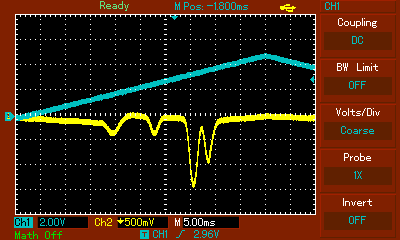
\includegraphics[width=0.9\linewidth]{build/V60_Bilder/spectrum.png}
      \caption{ Measurement of the Rb spectrum, through the combination of the Signals of the two photodiodes. The yellow line is the spectrum which shows the four peaks( here dips) of the Rb Atom. The blue line is the piezo current, which is triangular.    }
      \label{fig:sub1}
    \end{subfigure}%
    \begin{subfigure}{.5\textwidth}
      \centering
      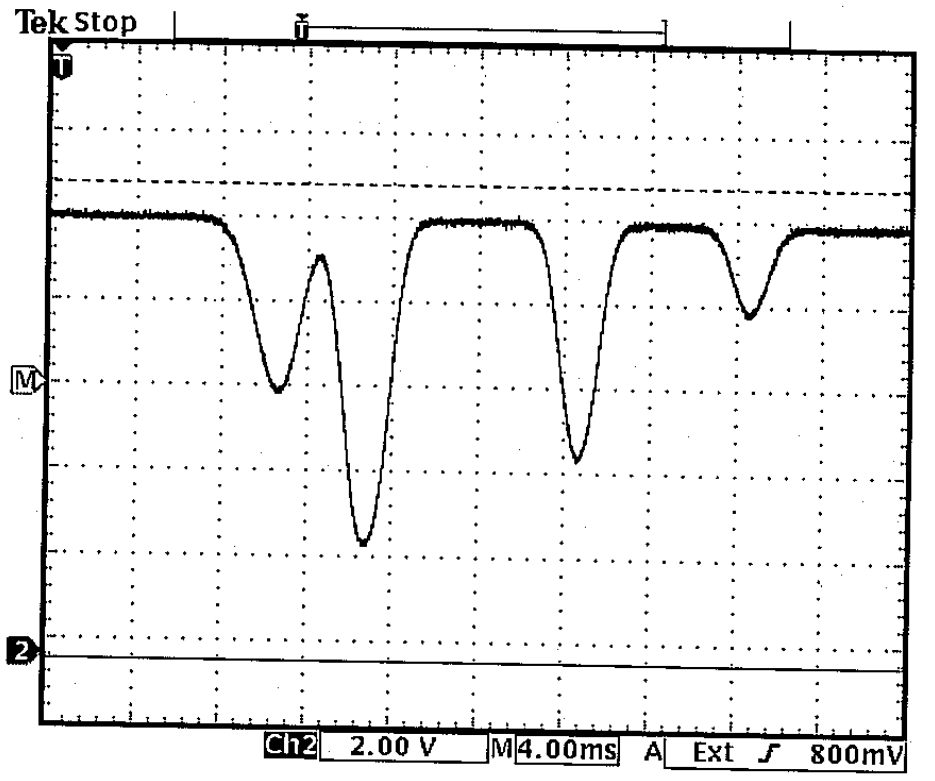
\includegraphics[width=.9\linewidth]{build/exp_spectrum.png}
      \caption{Expected spectrum for the Rb Atom, displayed for direct comparision and taken from the manual \cite{} }
      \label{fig:sub2}
    \end{subfigure}
    \caption{ Measurement(Left) of the Rb absorption spectrum and the expected(right) Spectrum. Note that the measured spectrum is inverted along the vertical axis. }
    \label{fig:spectrum}
 \end{figure}
